\documentclass{beamer}

\usepackage{soul}
\usepackage{graphicx}
\usepackage{tikz-cd}
\usepackage{tikz}
\usepackage{amssymb}
\usepackage{wasysym}
\usepackage{booktabs}
\usepackage{cases}
\usepackage{indentfirst}
\usepackage{graphicx}
\usepackage{adjustbox}
\newcommand{\new}[1]{\color{blue}#1\normalcolor}
\newcommand{\delete}[1]{}
\newcommand{\change}[1]{\color{black}#1\normalcolor}
\newcommand{\rev}[1]{\color{black}#1\normalcolor}


% VECTOR AND MATRIX NOTATION
\newcommand{\V}[1]{\boldsymbol{#1}}                 % vector notation
\newcommand{\M}[1]{\boldsymbol{#1}}
\newcommand{\Lop}[1]{\boldsymbol {\mathcal{#1}}}
\global\long\def\Ac{A_\text{cyto}}
\global\long\def\Pc{P_\text{cyto}}
\newcommand{\CDC}[1]{#1_{\text{c}}}
\newcommand{\6}[1]{#1_{\text{6}}}
\newcommand{\3}[1]{#1_{\text{3}}}
\newcommand{\CHIN}[1]{#1_{\text{ch}}}
\global\long\def\kon{k^\text{on}}
\global\long\def\koff{k^\text{off}}
\global\long\def\kf{k^+}
\newcommand{\Tot}[1]{#1^\text{(Tot)}}
\global\long\def\Dt{\partial_t}
\global\long\def\Dthat{\partial_{\hat{t}}}
\global\long\def\Dx{\partial_x}
\global\long\def\Dxhat{\partial_{\hat{x}}}
\global\long\def\MChinC{P_\text{cyto}}
\global\long\def\MChin{P_1}
\global\long\def\PChin{P_n}
\global\long\def\MAC{A_\text{cyto}}
\global\long\def\MA{A_1}
\global\long\def\PA{A_n}
\global\long\def\CDCy{C_\text{cyto}}
\global\long\def\CD{C}
\global\long\def\kp{k^\text{p}}
\global\long\def\kdp{k^\text{dp}}
\global\long\def\kI{k^\text{I}}
\global\long\def\kE{k^\text{E}}
\newcommand{\A}[1]{#1_A}
\newcommand{\Chin}[1]{#1_P}
\newcommand{\C}[1]{#1_C}
\global\long\def\DhatA{\hat{D}_A}
\global\long\def\KhatonA{\hat{K}^\text{on}_A}
\global\long\def\KhatoffA{\hat{K}^\text{off}_A}
\global\long\def\KhatfA{\hat{K}^\text{+}_A}
\global\long\def\KhatpA{\hat{K}^\text{p}_A}
\global\long\def\KhatdpA{\hat{K}^\text{dp}_A}
\global\long\def\DhatP{\hat{D}_P}
\global\long\def\KhatonP{\hat{K}^\text{on}_P}
\global\long\def\KhatonM{\hat{K}^\text{on}_M}
\global\long\def\KhatoffP{\hat{K}^\text{off}_P}
\global\long\def\KhatoffM{\hat{K}^\text{off}_M}
\global\long\def\KhatfP{\hat{K}^\text{+}_P}
\global\long\def\KhatpP{\hat{K}^\text{p}_P}
\global\long\def\KhatdpP{\hat{K}^\text{dp}_P}
\newcommand{\My}[1]{#1_M}
\newcommand{\R}[1]{#1_R}

\newcommand{\blue}[1]{\color{blue}#1\normalcolor}
\newcommand{\white}[1]{\color{white}#1\normalcolor}
\newcommand{\red}[1]{\color{red}#1\normalcolor}
\definecolor{ForestGreen}{RGB}{34,200,34}
\newcommand{\green}[1]{\color{ForestGreen}#1\normalcolor}

\newcommand\blfootnote[1]{%
  \begingroup
  \renewcommand\thefootnote{}\flushleft{\footnote{#1}}%
  \addtocounter{footnote}{-1}%
  \endgroup
}

\newcommand{\backupbegin}{
   \newcounter{finalframe}
   \setcounter{finalframe}{\value{framenumber}}
}
\newcommand{\backupend}{
   \setcounter{framenumber}{\value{finalframe}}
}

\usepackage{multimedia}
%\usepackage{palatino,paralist}
%
% Choose how your presentation looks.
%
% For more themes, color themes and font themes, see:
% http://deic.uab.es/~iblanes/beamer_gallery/index_by_theme.html
%
\mode<presentation>
{
  %\usetheme{Warsaw}      % or try Darmstadt, Madrid, Warsaw, ...
  \usecolortheme{dolphin} % or try albatross, beaver, crane, ...
  \usefonttheme{default}  % or try serif, structurebold, ...
  \setbeamertemplate{navigation symbols}{}
  \setbeamertemplate{caption}[numbered]
} 

\usepackage[english]{babel}
\usepackage[utf8x]{inputenc}

\title[Cell polarity dynamical system]{Maintenance phase biochemistry and contractility combine to encode a dynamically stable polarity state in the \emph{C elegans} zygote \vspace{-0.5 cm}}
\author[Ondrej Maxian, Cassandra Azeredo-Tseng, Ed Munro \& Others]{Ondrej Maxian, Cassandra Azeredo-Tseng, Ed Munro \& Others \vspace{-0.5 cm}}
%\institute[Courant Institute, NYU]{NYU MSG}
\date{Munro Lab Group Meeting \\ October 16, 2023}


\begin{document}

\addtobeamertemplate{navigation symbols}{}{%
    \usebeamerfont{footline}%
    \usebeamercolor[fg]{footline}%
    \hspace{1em}%
    \insertframenumber/\inserttotalframenumber
}

\begin{frame}
  \titlepage
\vspace{-0.5 cm}
\centering
\end{frame}

\begin{frame}{Cell polarization}
\end{frame}

\begin{frame}{\emph{C elegans} model system}
\begin{columns}
\begin{column}{0.6\textwidth}
Ingredients
\begin{itemize}
\item PAR proteins 
\begin{itemize}
\item aPARs (PAR-3, PAR-6, CDC-42)
\item pPARs (PAR-2, CHIN-1)
\end{itemize}
\item Actomyosin flows 
\end{itemize}
Wild type sequence
\begin{itemize}
\item Centrosomes $\rightarrow$ PAR-2 localized
\item Sperm cue $\rightarrow$ Myosin inhibition
\item Expansion of boundary to stable point (``establishment'')
\item ``Maintenance:'' boundary stays
\end{itemize}
\end{column}

\begin{column}{0.5\textwidth}
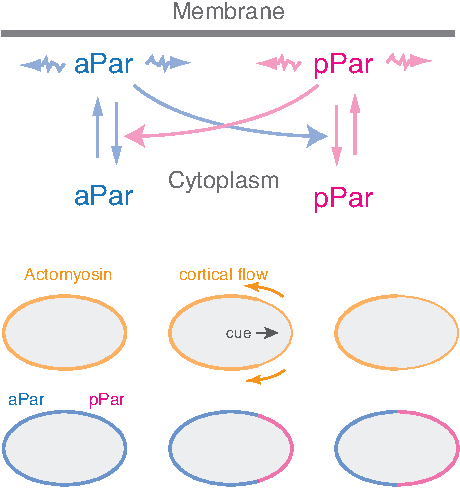
\includegraphics[width=\textwidth]{CElegansScheme-crop.pdf}
\end{column}
\end{columns}
\end{frame}

\begin{frame}{Movie: \emph{C elegans} wild type}
\end{frame}

\begin{frame}{The wild-type boundary is stable (the movie)}
Use CDK-1 (RNAi) to expand maintenance phase; boundary just sits there

This slide: movie

\end{frame}

\begin{frame}{The wild-type boundary is stable (the book)}
Plot of boundary position vs.\ time
\end{frame}

\begin{frame}{``Maintenance phase''}
Does ``maintenance'' maintain the current boundary in non wild-type embryos? 
\begin{itemize}
\item Establishment requires actomyosin 
\item Knockdown rho during establishment $\rightarrow$ no flows
\item Alternative: ECT-2 knockdown (GEF that activates Rho)
\item Both cases: local zone of PAR-2 enrichment remains
\end{itemize}

\begin{center}
\hspace{-0.75 cm} NMY-2::GFP  \phantom{O thou}  mCherry::PAR-2 \phantom{O thouth} Merge
\movie[width=\textwidth,loop]{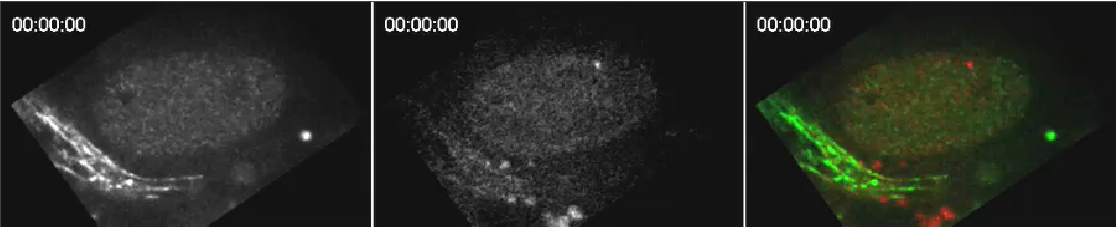
\includegraphics[width=\textwidth]{ZoniesFrame1.pdf}}{ZoniesNMYEct2.mov}
\end{center}

Results in exactly the same boundary position!
\begin{itemize}
\item Requires PAR-2, MRCK
\end{itemize}

\blfootnote{\tiny{Zonies et al. \emph{Development} (2010)}}
\end{frame}

\begin{frame}{The main questions}
How do the aPARs (PAR-3), pPARs (PAR-2) and actomyosin flows combine to yield a dynamically stable boundary position?
\begin{itemize}
\item Hypothesis 1: maintenance phase ``rescue'' = actomyosin instability (self-patterning) + mutual inhibition of PARs
\begin{itemize}
\item Uniform state is unstable
\item Fundamentally different from wild type
\end{itemize}
\item Hypothesis 2: ``rescue'' = pPAR/aPAR competition + pPAR inhibiting myosin 
\begin{itemize}
\item Uniform state stable
\item Small asymmetry amplified
\item Same as establishment phase mechanism
\end{itemize}
\end{itemize}

\end{frame}


\begin{frame}{Experimental and modeling program}
Hypothesis 1: maintenance phase ``rescue'' = actomyosin instability (self-patterning) + mutual inhibition of PARs
\begin{itemize}
\item Model myosin by itself
\item Infer parameters from experiments
\item Do we see self-amplification/instability?
\end{itemize}
Hypothesis 2: ``rescue'' = pPAR/aPAR competition + pPAR inhibiting myosin 
\end{frame}

\begin{frame}{Mathematics of stability}
$$\frac{dx}{dt}=\underbrace{f(x)}_\text{On rate}-\underbrace{g(x)}_\text{Off rate}$$
\begin{itemize}
\item Steady states: $f(x_s)=g(x_s)$
\end{itemize}
\begin{center}
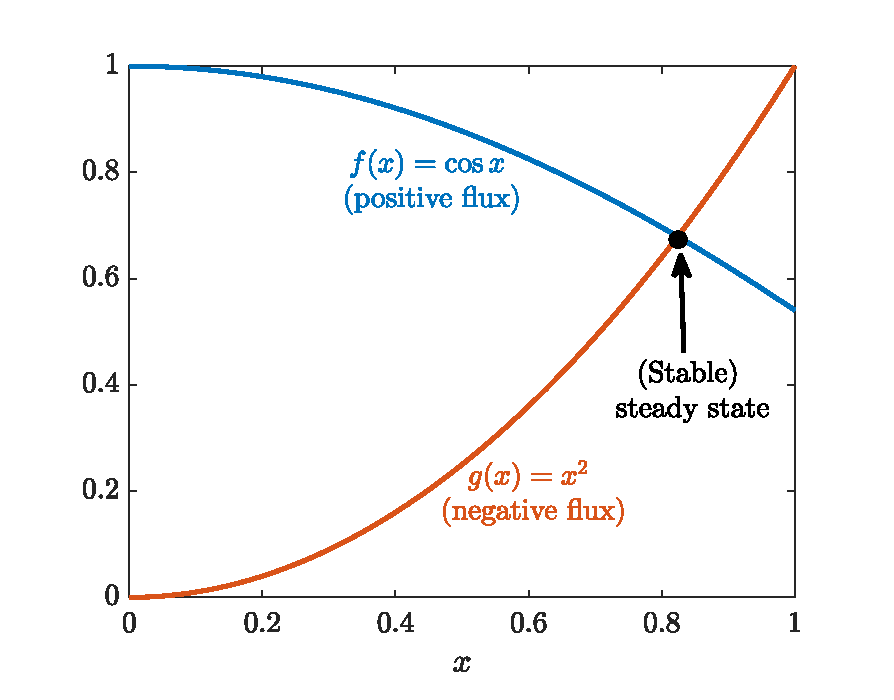
\includegraphics[width=0.6\textwidth]{FluxExample.eps}
\end{center}
\begin{itemize}
\item Stable steady state $f(x_s^+) < g(x_s^+) < 0$,  $f(x_s^-)  > g(x_s^-)$
\item Perturb off the steady state and get pushed back to it
\end{itemize}
\end{frame}

\begin{frame}{Model of the \emph{C elegans} embryo}
\centering
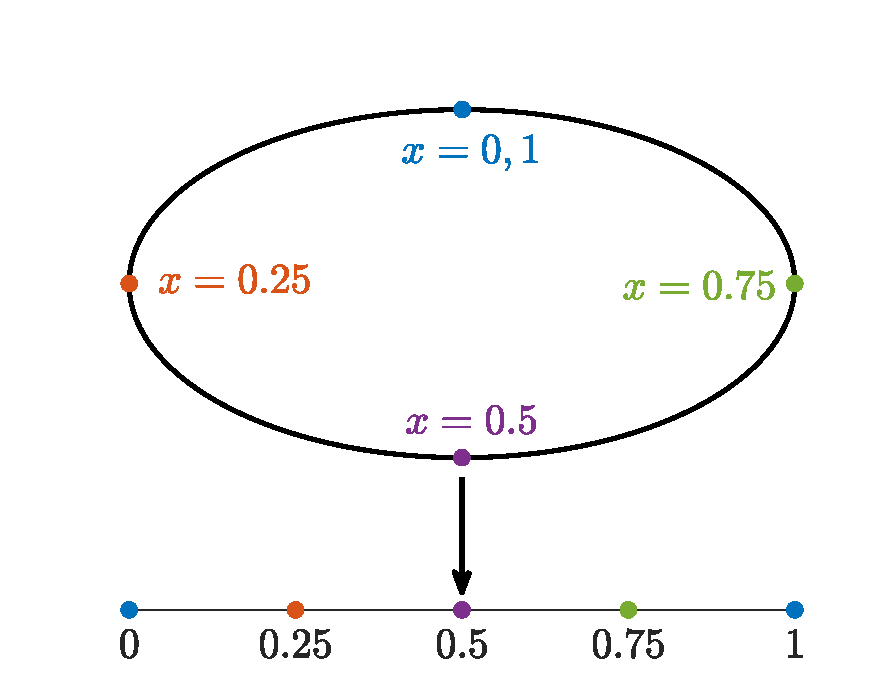
\includegraphics[width=0.7\textwidth]{ModelGeo.eps}

\end{frame}

\begin{frame}{Myosin dynamics}
\begin{gather*}
\Dt M + \underbrace{\Dx \left(v M\right)}_\text{Advection} = \underbrace{D_M \Dx^2 M}_\text{Diffusion} +\underbrace{\My{\kon}M_\text{cyto}}_\text{On flux} - \underbrace{\My{\koff} M}_\text{Off flux} \\
M_\text{cyto} =  1 - \int_0^1 M(x) \, dx \\
\underbrace{\gamma v}_\text{Drag force} = \underbrace{\eta \Dx^2 v}_\text{Viscous stress} + \underbrace{\Dx \sigma_a(M)}_\text{Active stress}
\end{gather*}
\begin{itemize}
\item Strong enough flows $\rightarrow$ self patterning
\item Only unknown: stress vs.\ myosin relationship 
\end{itemize}

\blfootnote{\tiny{Bois et al. \emph{PRL} (2011)}}
\end{frame}

\begin{frame}{Stable and unstable myosin dynamics}
\begin{center}
\movie[width=\textwidth,loop]{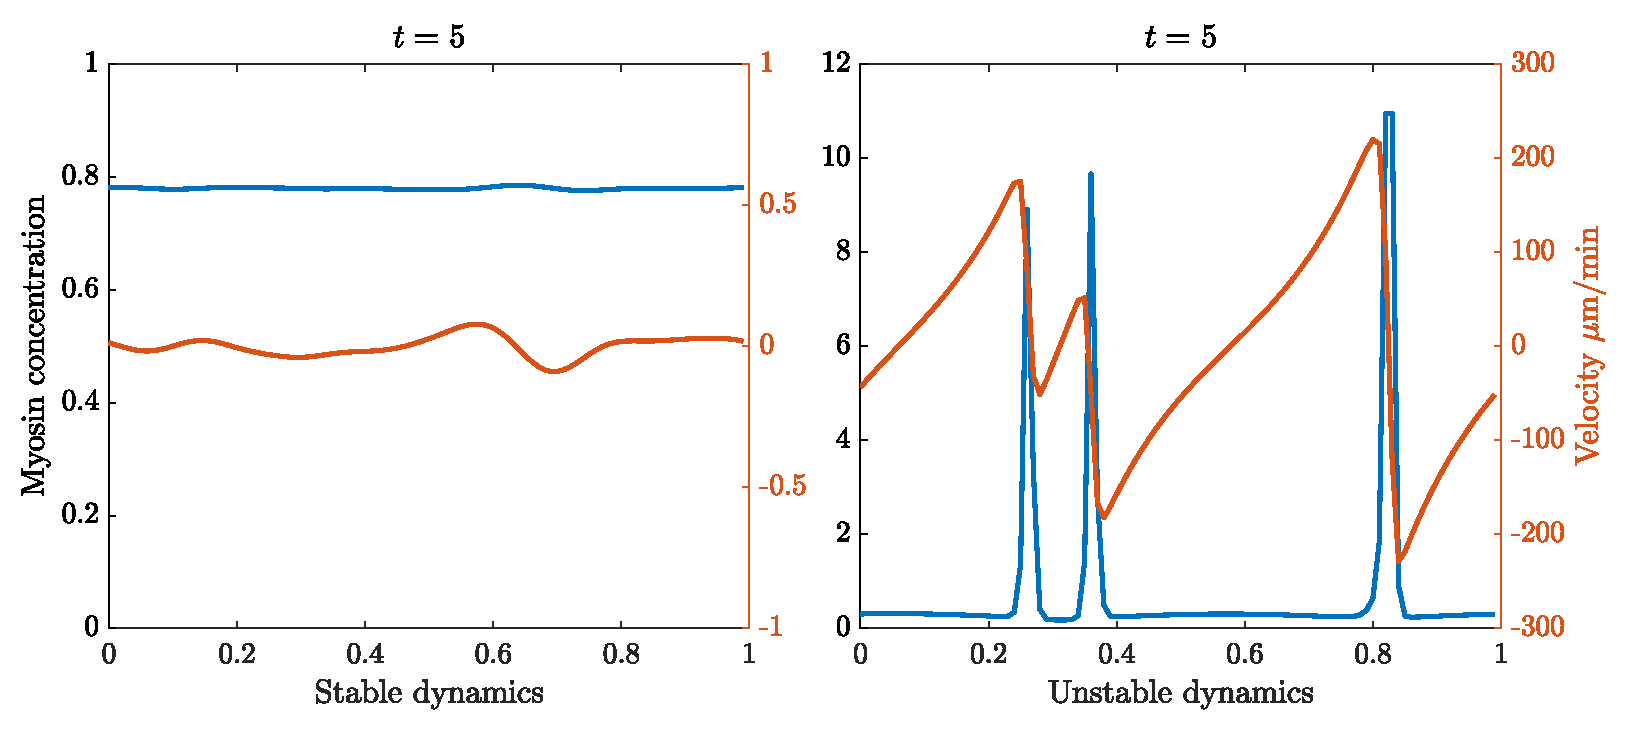
\includegraphics[width=\textwidth]{MyosinStill.eps}}{MyosinDynamics.mp4}
\end{center}
Unstable flow patterns characterized by unphysical speeds
\end{frame}

\begin{frame}{Inferred myosin velocity}
\begin{center}
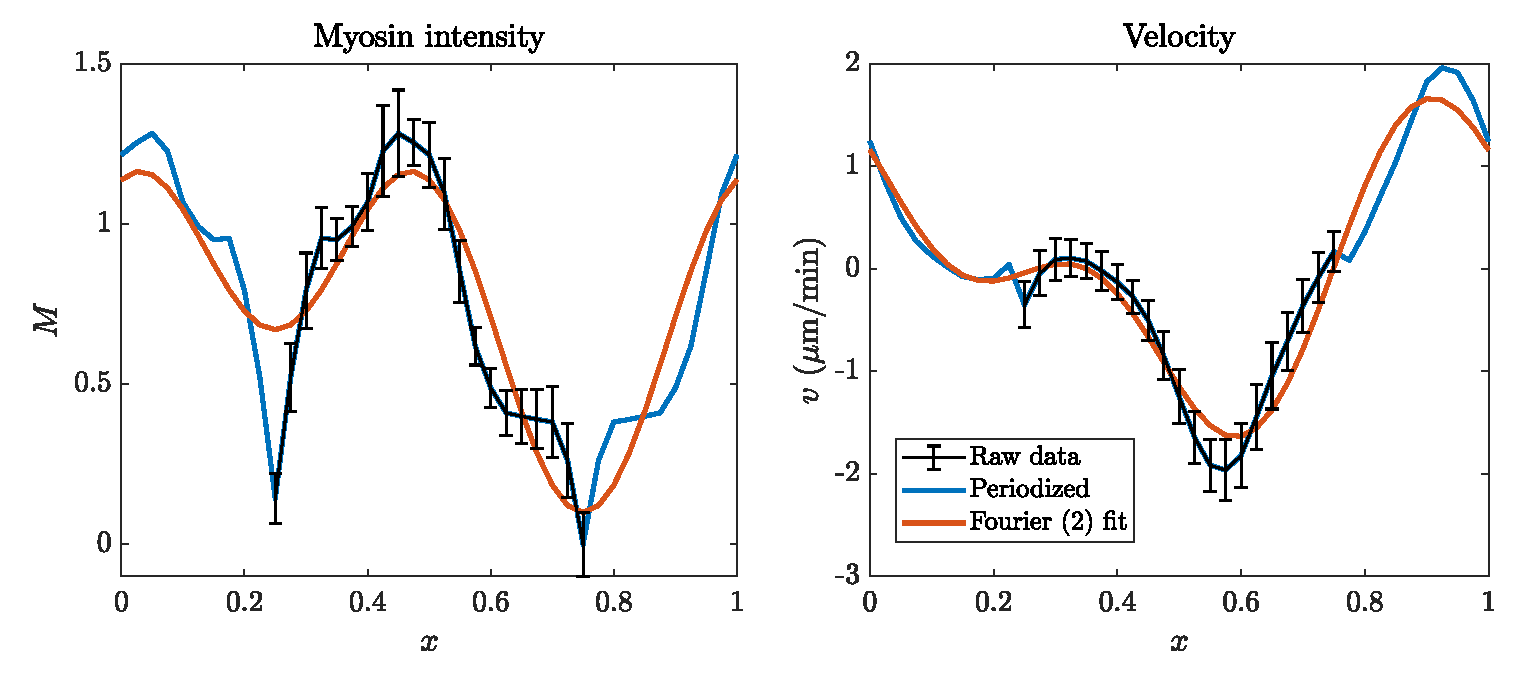
\includegraphics[width=\textwidth]{MyosinFittingPres.eps}
\end{center}
Solve $$\gamma v = \eta \Dx^2 v+ \Dx \sigma_a(M)$$
to get active stress $\sigma_a(M)$

\blfootnote{\tiny{Sailer et al. \emph{Dev.\ Cell} (2010)}}
\end{frame}

\begin{frame}{Inferred myosin dynamics}
\begin{center}
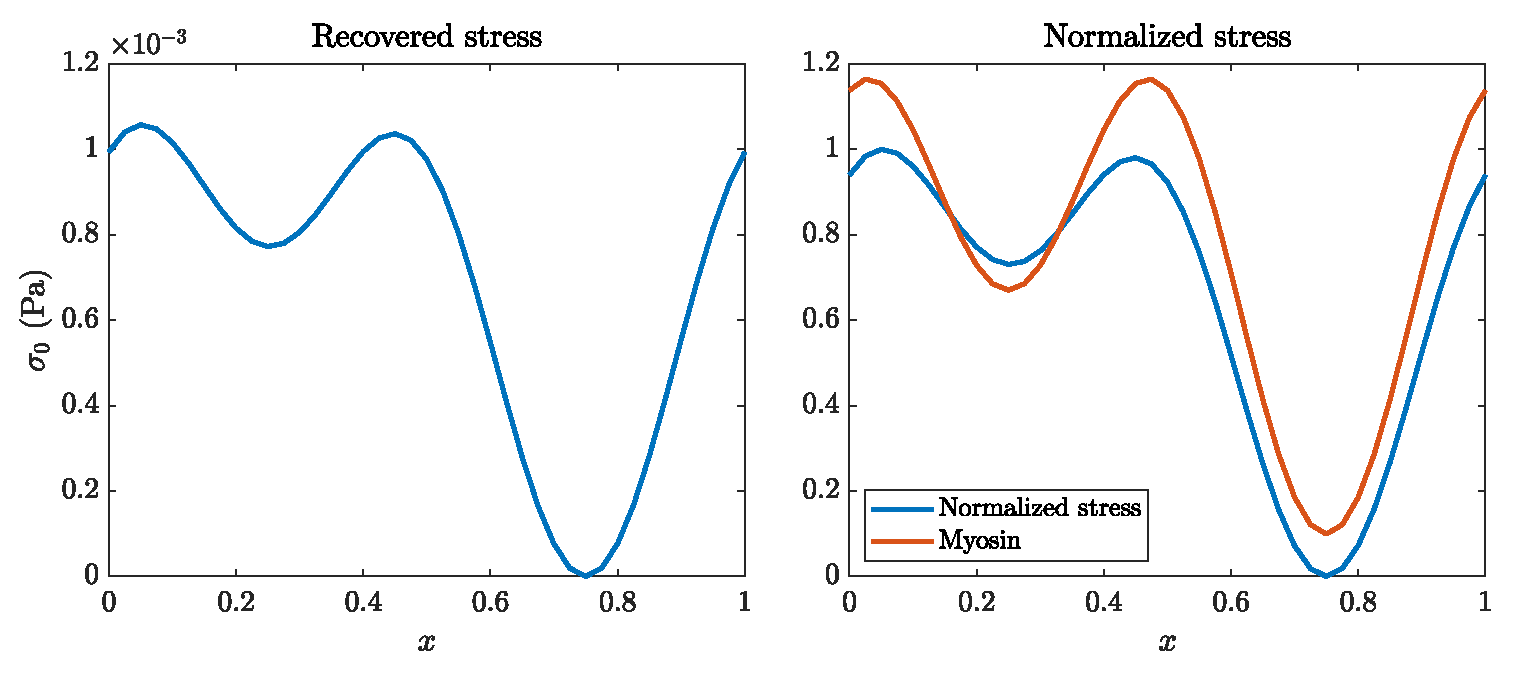
\includegraphics[width=\textwidth]{MyosinStressPres.eps}
\end{center}
Active stress roughly proportional to myosin intensity
\begin{itemize}
\item $\sigma_a \approx \left(1.1 \times 10^{-3}\right) M$ 
\item Not even close to strong enough for instability! 
\item Never see sharp peaks in arbitrary places
\item Despite appearances, \emph{no spontaneous symmetry breaking}
\item System has 2 steady states
\end{itemize}
\end{frame}



\begin{frame}{Experimental and modeling program}
\st{Hypothesis 1: maintenance phase ``rescue'' = actomyosin instability (self-patterning) + mutual inhibition of PARs}

\vspace{0.5 cm}

Hypothesis 2: ``rescue'' = pPAR/aPAR competition + pPAR inhibiting myosin 
\begin{itemize}
\item Start with model of aPAR/pPAR competition
\item Add myosin on top
\end{itemize}
\end{frame}

\begin{frame}{PAR competition gives contracted boundary}
PAR asymmetries stable by themselves without flows

\begin{columns}
\begin{column}[T]{0.49\textwidth}
\begin{itemize}
\item Wild-type embryos with MRCK knockout $\rightarrow$ boundary expands, but still asymmetric
\item ECT-2 (RNAi) embryos: MLC-1 (RNAi) produces mutually inhibitory zones of PAR-2 and PAR-3
\item Suggests that mutual antagonism encodes one steady state
\end{itemize}
\end{column}
\begin{column}[T]{0.49\textwidth}
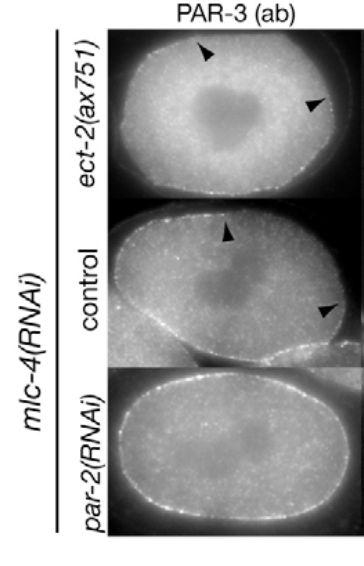
\includegraphics[width=0.9\textwidth]{ZoniesNoMyosin.png}
\end{column}
\end{columns}

\blfootnote{\tiny{Zonies et al. \emph{Development} (2010)}}
\end{frame}

\begin{frame}{First model for mutual inhibition}
First model: mutual inhibition of proteins, mass-action kinetics
\begin{align*}
\Dt A &= D_P \Dx^2 A + \kon_A A_\text{cyto} - \koff_A A -r_\text{AP} AP \\
\Dt P &= \underbrace{D_P \Dx^2 P}_\text{Diffusion} + \underbrace{\kon_P P_\text{cyto} - \koff_P P}_\text{Binding/unbinding} \underbrace{-r_\text{AP} AP}_\text{Mutual inhibition}
\end{align*}
\begin{itemize}
\item \emph{One} stable steady state!
\item Need a way to generate \emph{bistability}
\end{itemize}
\end{frame}

\begin{frame}{The Grill workaround}
\begin{center}
 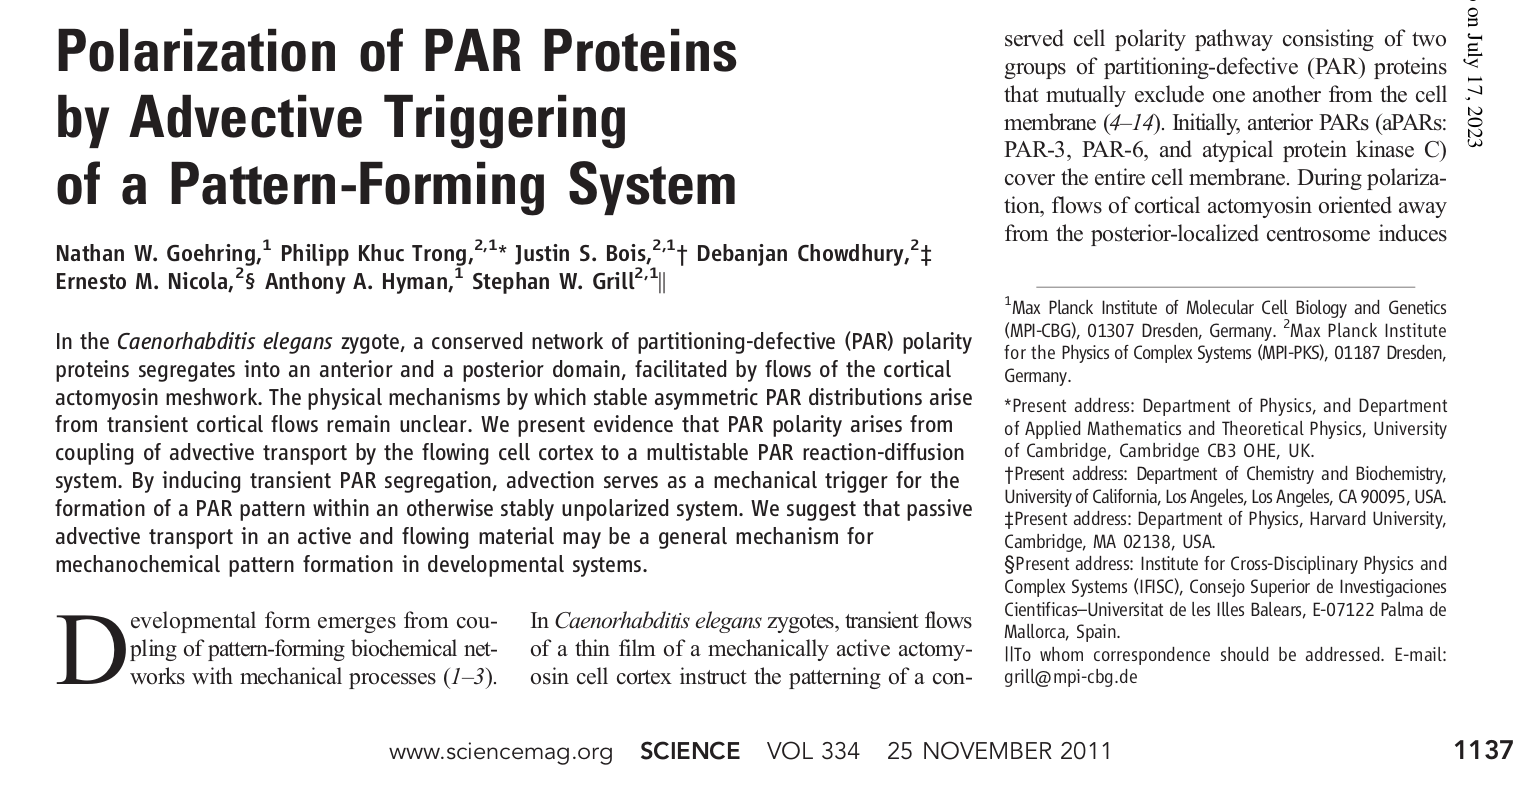
\includegraphics[width=\textwidth]{GrillTitle.png}
\end{center}
\end{frame}

\begin{frame}{The Grill workaround}

\begin{center}
\vspace{-3 cm}
 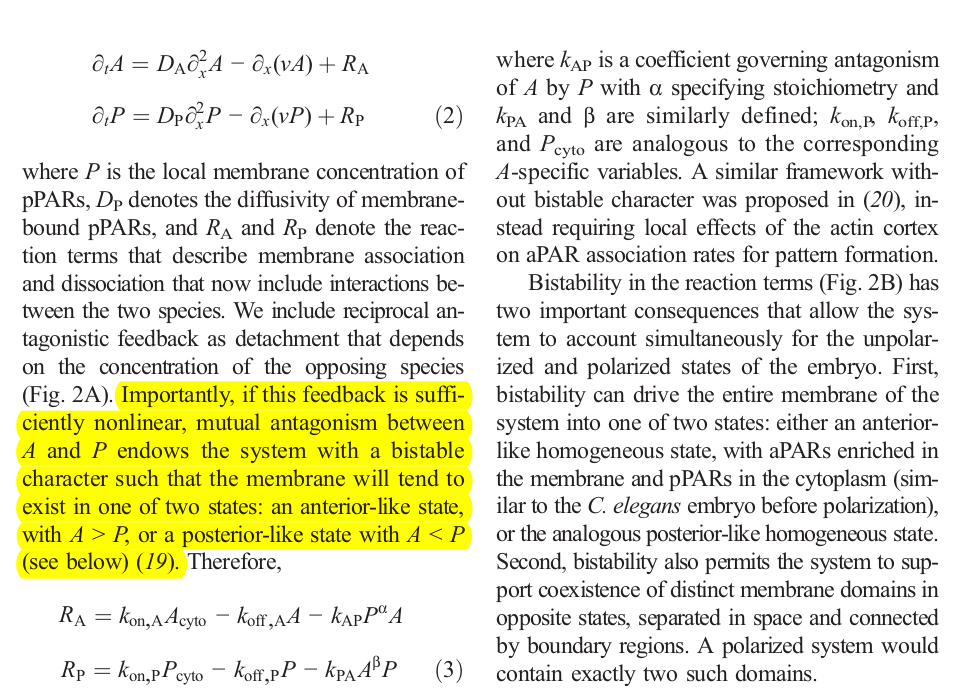
\includegraphics[width=\textwidth]{GrillRxn.png}
\end{center}

\visible<2->{
\vspace{-7 cm}
\begin{center}
 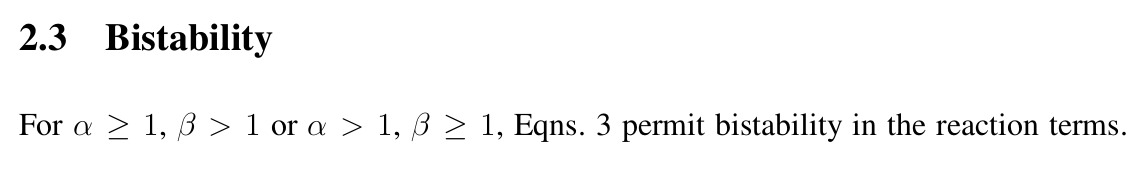
\includegraphics[width=\textwidth]{GrillChoice.png}
\end{center}}
\end{frame}

\begin{frame}{The Charlie-Ed solution: PAR-3}
Important experimental observations
\begin{itemize}
\item PAR-3 stable by itself
\item All asymmetries are lost without it
\item Higher recruitment rate when more monomers attached
\item Oligomerization
\item Evidence that feedback + oligomerization $\rightarrow$ stability
\end{itemize}
\end{frame}

\begin{frame}{PAR-3 model}
Pinned boundary position
\end{frame}

\begin{frame}{Incorporating PAR-2}
Mass action kinetics $\rightarrow$ different zones

Boundary can only make it so far! Need another piece
\end{frame}

\begin{frame}{Experimental and modeling program}
Hypothesis:``rescue'' = pPAR/aPAR competition + pPAR inhibiting myosin 
\begin{itemize}
\item Start with model of aPAR/pPAR competition
\item Add myosin on top
\end{itemize}
\end{frame}

\begin{frame}{Full model: PAR-2/PAR-3/Myosin}
Dynamics of myosin
\begin{itemize}
\item Inhibited locally by pPARs
\item Transports everything (including itself!)
\end{itemize}
\end{frame}

\begin{frame}{Steady states}
\end{frame}

\begin{frame}{Contractility on/off}
Start with mutual aPAR/pPAR inhibition. Let equilibrate. Add contractility. Let equilibrate. Turn off contractility. Should go back to first position
\end{frame}

\begin{frame}{Remaining issues}
What causes boundary to stop?
\begin{itemize}
\item This model: 
\item Experiment: something different?
\end{itemize}
Clear that flow profiles do not match
\end{frame}

\begin{frame}{Branched actin as a brake on contractility}
Cassandra's movies on arp 2/3 knockout

Idea: flow profile here should be same as original model

Then add branched actin to the model to complete the story

\end{frame}



\iffalse
\begin{frame}{Computational rheology in dynamic cross-linked networks}
\centering
\movie[width=0.48\textwidth]{
 \includegraphics[width=0.48\textwidth]{RelaxationTurnover5_478.png}
}{ShearTurnover5.mp4}
\movie[width=0.48\textwidth]{
 \includegraphics[width=0.48\textwidth]{RelaxationTurnover10_478.png}
}{ShearTurnover10.mp4}
\newline \phantom{x} \qquad $\tau_f/\tau_c \approx 0.3$ \qquad \qquad \qquad \qquad \quad $\tau_f/\tau_c \approx 0.7$ 
\newline ``Meshwork'' \qquad \qquad \qquad \qquad \quad ``B-In-M''
\end{frame}
\fi



\end{document}
